\documentclass[conference]{IEEEtran}
\usepackage[utf8]{inputenc}
\usepackage[T1]{fontenc}
\usepackage{cite}
\usepackage{amsmath,amssymb,amsfonts}
\usepackage{algorithm}
\usepackage{algpseudocode}
\usepackage{graphicx}
\usepackage{booktabs}
\usepackage{multirow}
\usepackage{xcolor}
\usepackage{tikz}
\usetikzlibrary{arrows.meta,positioning,shapes.geometric,fit,calc}
\usepackage{url}
\usepackage[hidelinks]{hyperref}
\graphicspath{{figures/}}

\emergencystretch=2em

\begin{document}

\title{When Does Federation Help an Edge Payload Classifier? A Measurement Study with an Authenticated Robust Aggregator}

\author{\IEEEauthorblockN{Alessandro De Martini}
\IEEEauthorblockA{\textit{Department of Information Systems and Technology} \\
\textit{Mid Sweden University (MIUN)}\\
Sundsvall, Sweden \\
alessandro.demartini@miun.se}
}

\maketitle

\begin{abstract}
Industrial gateways inspect HTTP requests from sites whose benign traffic differs, while data-governance rules may keep those requests on site. We ask when federating a lightweight payload classifier, a logistic regression over hashed character trigrams, across such sites helps, and at what cost and security limit. When two sites differ in benign profile and face the same attacks, federated averaging matches the best isolated model within seed variation (ROC-AUC 0.9947 vs.\ 0.9938 over eight seeds on exact-unique splits) and beats the silo with the wrong benign profile (0.9859). With near-duplicate payloads grouped, it is indistinguishable from pooled training of the same model and not better than the test-optimal silo. When sites differ in attack mix, federation lifts the weaker silo but stays below the stronger one. FedProx does not improve on FedAvg, and in a rerun of the recipe gradient-boosted trees on the same features reach ROC-AUC 0.989 against 0.969 for the linear model. The evidence for deployment is adverse: on CSIC~2010 the gateway's maximum-over-contexts rule flags all 72{,}000 normal requests, because the model scores the constant \texttt{User-Agent} header above threshold, and scoring payload contexts only still flags 19\% at the deployed threshold. We also describe a prototype aggregator that authenticates updates with HMAC-SHA256 and aggregates them by coordinate-wise median behind a norm gate. In simulation with eight seeds and 40\% malicious clients, the median keeps ROC-AUC at 0.90--0.97, but its false-positive rate at the deployed threshold rises to 0.24--0.67 under four of five attacks. The live update channel is plain HTTP; ML-KEM-512 was benchmarked as a component and is not integrated. A fixed 1{,}040-byte update cuts cloud-bound traffic by 98.88\% at the deployed 15\,s synchronisation interval and 452 requests per second, relative to shipping every request payload.
\end{abstract}

\begin{IEEEkeywords}
Federated Learning, Web Application Firewall, Non-IID Data, Byzantine-Robust Aggregation, Edge Computing, Industrial IoT
\end{IEEEkeywords}

\section{Introduction}
\label{sec:intro}

A gateway that terminates HTTP traffic for web front-ends and device APIs is the natural place to inspect requests at the industrial edge. Most deployed inspection is signature-based~\cite{modsecurity,roesch1999,suricata}: rules are curated by hand and generalise poorly to polymorphic or unseen payloads. A learned classifier would adapt, but it needs traffic, and in an Industrial Data Space such as Gaia-X~\cite{gaiax2021} the requests are the very thing that cannot leave the site: they embed proprietary API queries, tokens and process telemetry. Federated learning~\cite{mcmahan2017} avoids moving the data by training on each gateway and exchanging only model parameters, so that a site can benefit from an attack first seen elsewhere without any request leaving either site.

Whether that benefit materialises at a given site is less obvious than the framing suggests. Federated averaging can converge to a worse solution than local training when client objectives diverge~\cite{li2020convergence}, and what ``diverge'' means for web traffic is specific. Two sites may face different attack campaigns against the same kind of application, or the same attacks against applications whose benign requests look nothing alike, a web front-end with path words against an API with JSON endpoints. These are different kinds of non-IID data, and a classifier that must separate benign from malicious is affected by them differently. We found no study that separates the two for a federated WAF, although the search behind that statement was bounded (Section~\ref{sec:background}).

Our question is therefore: \emph{when does federating a lightweight HTTP payload classifier across sites with different benign profiles or attack mixes help, and at what cost and security limit?} We study a deliberately small model, a logistic regression over hashed character trigrams with a fixed-size update, because it fits an ARM gateway and because its simplicity keeps the comparison between federated and isolated training interpretable. $K$ gateways each hold traffic that must stay on site, and one cloud aggregator combines their parameters. Evaluation is on unique-payload-disjoint splits, at a matched false-positive budget, over eight seeds. The prototype is a payload-scoring component for such a gateway. It does not identify or authenticate the requester, so it is one input to an access decision and not a zero-trust architecture.

\subsection{Contributions}
\begin{enumerate}
    \item \textbf{A measurement of when federation helps.} Over two constructed heterogeneity axes and two feature sets, federation lifts the weaker silo and reduces cross-domain false positives, matches the best silo on aggregate ROC-AUC within seed variation when sites differ in benign profile, and does not reliably exceed the best silo on SQL-injection recall (Section~\ref{sec:evaluation}). We also report what an operating-point-aware evaluation of the gateway on CSIC~2010 shows: the deployed scoring rule flags all normal requests in that corpus.
    \item \textbf{A prototype authenticated robust aggregator.} Updates carry HMAC-SHA256 tags with timestamps and single-use nonces, are checked against an enrolment list, and are aggregated by coordinate-wise median after dimension and norm checks. In simulation with 2 of 7 clients sign-flipping, the median retains ROC-AUC 0.984 against 0.263 for averaging. The threat model, the controls and their limits, including a plain-HTTP live channel with ML-KEM benchmarked only as a component, are set out in Sections~\ref{sec:system} and~\ref{sec:security}.
    \item \textbf{Cost and dataset-construction lessons.} A fixed 1{,}040-byte update reduces cloud-bound traffic by 98.88\% at the deployed 15\,s interval (75.0\% over a 20-round training run, where every round and both directions are charged). Two construction errors, resampling before splitting on unique payloads and rendering the two classes with different request templates, inflate results on this task and are documented with their effect.
\end{enumerate}
What remains open is how far a result on two clients and public payload lists can be pushed, and which parts of earlier work already answer pieces of the question.

\section{Background and Related Work}
\label{sec:background}

Four bodies of work bear on the question left open by the introduction: per-request enforcement at a gateway, federated optimisation under heterogeneity, payload representation, and the security of the update channel. Statements below that something has not been done are limited to the searches described in the positioning subsection.

\subsection{Zero-Trust Architecture}
Zero trust drops the assumption that a request is benign because it originates inside the network perimeter. NIST SP~800-207 formalises this: no implicit trust is granted by network location, and every access decision is made per request, based on the observable state of the requester and the resource~\cite{nist800207}. Google's BeyondCorp was an early large-scale deployment of the idea~\cite{beyondcorp}. The architecture separates a policy decision point from policy enforcement points that sit in front of each resource.

Here the enforcement point is a gateway-resident Web Application Firewall (WAF), and the only decision signal is a learned score over the request payload. Requester identity and posture, which NIST assigns to the policy decision point, are outside the prototype; it supplies one input to such a decision. The open problem is how to keep that decision function current against new payloads without centralising the traffic it is trained on. Signature engines such as Snort~\cite{roesch1999} depend on curated rules and cannot adapt on their own. Sommer and Paxson also caution that learned detectors in network security cannot assume a closed world, because the benign class is site-specific and attacks keep changing~\cite{sommer2010}. That observation motivates testing the benign-traffic profile as a heterogeneity axis, separately from the attack mix.

\subsection{Federated Learning}
Federated learning (FL) trains a shared model while data stays on the participants. In Federated Averaging (FedAvg), each client runs local optimisation and the server averages the returned parameters, weighted by local sample count~\cite{mcmahan2017}. Kairouz \textit{et al.} survey the open problems~\cite{kairouz2021}; those most relevant here are statistical heterogeneity, communication cost, and adversarial participants.

\paragraph{Heterogeneity.}
When client distributions differ, local optima diverge. Li \textit{et al.} prove that FedAvg converges more slowly on non-IID data~\cite{li2020convergence}, and FedProx adds a proximal term to stabilise training under such heterogeneity~\cite{li2020fedprox}. We do not use a proximal term; we instead study which \emph{kind} of heterogeneity helps or hurts a plain FedAvg aggregation.

\paragraph{Privacy.}
Raw data never leaves a client, but updates are not free of information: gradients can be inverted to reconstruct training inputs~\cite{zhu2019}. Differentially private training with clipping and noise~\cite{abadi2016} and cryptographic secure aggregation~\cite{bonawitz2017} are the standard mitigations. Mothukuri \textit{et al.} survey attacks and defences~\cite{mothukuri2021}.

\paragraph{Byzantine robustness.}
A compromised client can upload arbitrary parameters. Krum~\cite{blanchard2017}, coordinate-wise median and trimmed mean~\cite{yin2018} replace the mean with a robust statistic, under the assumption that honest clients outnumber malicious ones. These rules are not a complete defence: Fang \textit{et al.} construct local model-poisoning attacks that degrade them~\cite{fang2020}.

\paragraph{Communication.}
Update size dominates cost on constrained links. Quantisation and encoding schemes such as QSGD reduce it~\cite{alistarh2017}. A fixed-width feature map attacks the same problem differently, by making the model, and hence the update, a constant size.

\paragraph{FL for IoT security.}
FL has been applied to anomaly detection on IoT gateways, for example DIoT, which learns per-device-type communication profiles federatedly~\cite{nguyen2019diot}, and is surveyed for IoT in general by Nguyen \textit{et al.}~\cite{nguyen2021}. Federated detection of web attacks has been studied for XSS on edge devices, with non-IID data as a stated concern, but we did not find work that separates attack-campaign heterogeneity from benign-profile heterogeneity for a federated payload classifier.

\subsection{Behavioural and \texorpdfstring{$n$}{n}-gram Profiling of Payloads}
Behavioural profiling models what normal input looks like and scores deviations. Forrest \textit{et al.} used short sequences of system calls as a signature of ``self'' for processes~\cite{forrest1996}. For network and web traffic, PAYL models the byte-frequency distribution of payloads~\cite{wang2004payl}, and Kruegel and Vigna model request attributes of web applications~\cite{kruegel2003}. Character $n$-gram statistics are a long-standing representation in text classification~\cite{cavnar1994}, and they transfer directly to HTTP payloads because injection attacks have distinctive local character patterns (for example quote--keyword--comment sequences in SQL injection, or angle-bracket--tag sequences in XSS).

An explicit $n$-gram vocabulary grows with the traffic seen, which would make the model size, and every synchronisation payload, unbounded. The hashing trick maps $n$-grams into a fixed number of buckets without a vocabulary~\cite{weinberger2009}. Our feature map hashes character trigrams ($n=3$) into 256 buckets with a polynomial rolling hash, $\ell_2$-normalises the bucket counts, and appends three scaled syntactic scalars (length, count of non-alphanumeric characters, Shannon entropy), giving a 259-dimensional vector (\texttt{fedzta\_features.py}). The same module runs on cloud and edge so both sides bucket identically. Because the map is fixed and cheap to compute, a linear classifier suffices on the gateway. Hashed $n$-gram payload models are also known to be evadable by an attacker who shapes the byte statistics of an attack~\cite{fogla2006}, a limitation the linear model inherits and this study does not test.

\subsection{Post-Quantum Key Encapsulation for the Weight Channel}
Model parameters are valuable, and an adversary who records the channel today may decrypt it later. Shor's algorithm breaks the factoring and discrete-logarithm problems that underlie RSA and elliptic-curve Diffie--Hellman~\cite{shor1997}, so key exchange that relies on them is exposed to this ``store now, decrypt later'' strategy. Post-quantum cryptography replaces them with problems believed hard for quantum computers~\cite{bernstein2017}.

NIST has standardised two lattice-based schemes derived from the CRYSTALS submissions. \textbf{ML-KEM} (FIPS~203)~\cite{fips203}, derived from CRYSTALS-Kyber~\cite{bos2018kyber}, is a key-encapsulation mechanism: the receiver publishes a public key, the sender encapsulates a fresh shared secret under it and returns a ciphertext, and the receiver decapsulates. The shared secret then keys a symmetric cipher for the payload. \textbf{ML-DSA} (FIPS~204)~\cite{fips204}, derived from CRYSTALS-Dilithium~\cite{ducas2018dilithium}, is the corresponding digital signature scheme.

The prototype includes a standalone ML-KEM-512 demonstration, the smallest parameter set, using the \texttt{pqcrypto} Python bindings. The cloud side (\texttt{cloud\_pqc.py}) generates a keypair and serves the public key; the edge side (\texttt{edge\_pqc.py}) fetches it and encapsulates a shared secret. That secret is not yet used to encrypt the live update and weight endpoints, which carry HMAC-authenticated JSON over plain HTTP. Authentication is separate: each gateway is enrolled with a 256-bit secret and tags updates with HMAC-SHA256 (\texttt{fedzta\_auth.py}), using only the Python standard library. A MAC is not a signature; ML-DSA would replace the shared secret with per-gateway public keys at the price of an extra edge dependency, and is not evaluated here.

\subsection{Positioning}
The search behind the novelty statements in this paper was bounded: a small number of web and preprint searches on federated WAF and web-attack detection, post-quantum federated learning, and Byzantine-robust aggregation, plus the authors' knowledge of the literature. It was not a systematic review, and absence of a hit means only that none was found. Within that bound, each ingredient exists elsewhere: federated detection of injection attacks, hashed $n$-gram payload models, robust aggregation, and post-quantum key exchange on small devices, with recent preprints combining post-quantum protection and Byzantine-robust federated learning for industrial intrusion detection. The measurement we found no counterpart for is the controlled comparison of benign-profile and attack-mix heterogeneity for a payload classifier under unique-payload-disjoint evaluation, and the care needed for that comparison follows the general warnings on dataset construction in security machine learning~\cite{arp2022}. The robustness we examine is that of the baseline rules above against a naive adversary, and no formal privacy guarantee is claimed. The system that carries out the comparison is described next.

\section{System and Method}
\label{sec:system}

The question of when federation helps needs a classifier cheap enough to run on every request at a gateway and small enough that exchanging it costs next to nothing. The system built to test this has two roles. An \emph{edge gateway} scores HTTP requests locally with a linear model and never transmits payloads. A \emph{cloud aggregator} accepts MAC-tagged parameter updates from enrolled gateways, combines them, and returns a global model. Figure~\ref{fig:architecture} shows the flow. The gateway is a web application firewall (WAF) enforcement point. It can sit inside a zero-trust deployment, where it supplies one per-request check on payload content, but it does not establish requester identity or device posture and is not itself a zero-trust architecture. Trust assumptions, adversaries and the limits of each control are stated once, in Section~\ref{sec:sec-threat}; this section describes mechanisms only.

\begin{figure}[t]
\centering
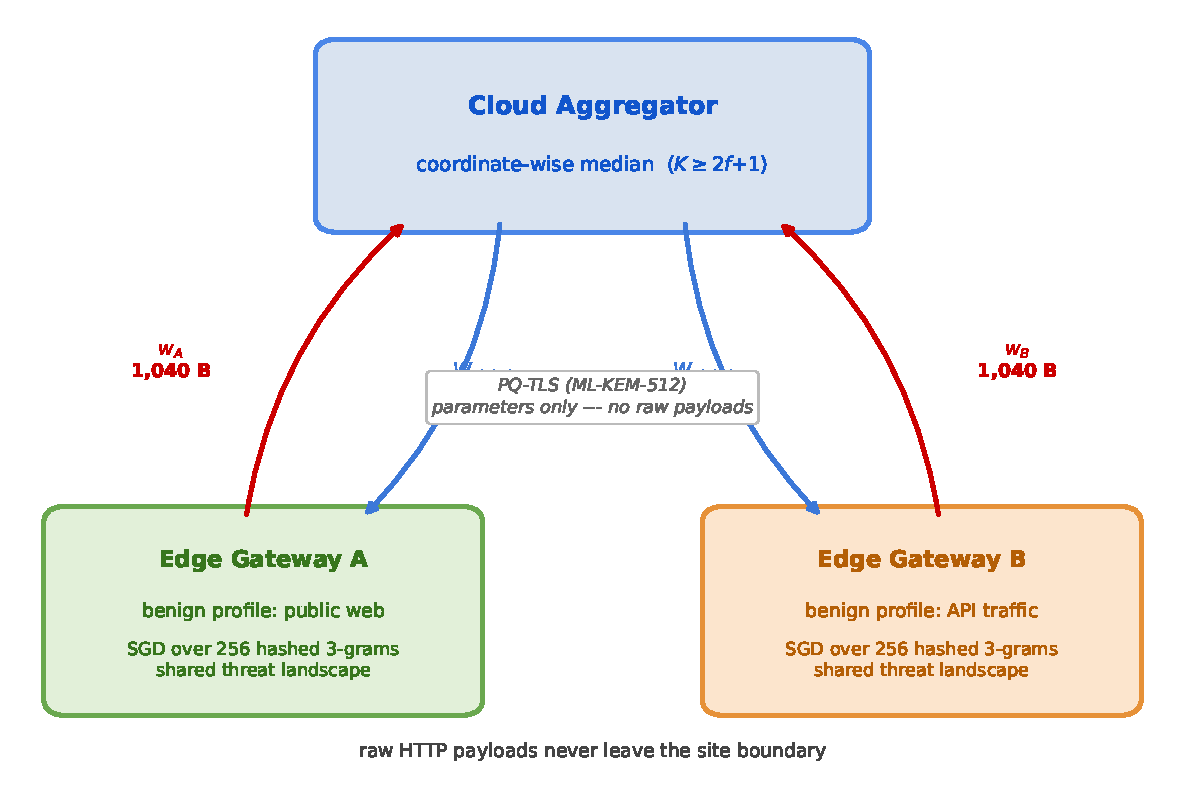
\includegraphics[width=\linewidth]{figures/fl_architecture.pdf}
\caption{System architecture. Edge gateways score requests locally and upload MAC-tagged weight vectors over plain HTTP; the cloud aggregator authenticates, gates and aggregates them. Raw traffic stays at the edge.}
\label{fig:architecture}
\end{figure}

\subsection{Features and Classifier}
\label{sec:sys-features}
Feature computation lives in one module, \texttt{fedzta\_features.py}, imported by the gateway, the aggregator and the profiler so that every party buckets n-grams identically. The unit that is featurised is a \emph{context} $P$: one string such as a path, a query string, a header value or a body. Each context maps to $\mathbf{x}(P)\in\mathbb{R}^{D+3}$ with $D=256$, i.e.\ $259$ dimensions:
\begin{equation}
\mathbf{x}(P) = \big[\, \hat{\mathbf{h}}(P) \;\big|\; \tfrac{|P|}{100} \;\big|\; \tfrac{s(P)}{20} \;\big|\; \tfrac{H(P)}{5} \,\big].
\end{equation}
Here $\hat{\mathbf{h}}(P)$ is the $\ell_2$-normalised histogram of lower-cased character trigrams hashed into $D$ buckets by a polynomial rolling hash (multiplier $131$, $32$-bit state), $s(P)$ counts non-alphanumeric characters, and $H(P)$ is the Shannon entropy of the character distribution. The polynomial hash replaced MD5 for speed on the Cortex-A72 (0.242\,ms versus 0.404\,ms per request in an earlier profiling run). The scaling constants $(100,20,5)$ are fixed a priori, so no scaler is shipped to the edge and no test statistics reach training.

The classifier is logistic regression, $p(\mathbf{x})=\sigma(\mathbf{w}^\top\mathbf{x}+b)$, with the logit clipped to $[-250,250]$. The model has $259$ coefficients and an intercept, $1{,}040$ bytes in single precision, which is also the size of one synchronisation payload.

\subsection{Training Unit and Scoring Unit}
\label{sec:sys-units}
Training and inference operate on different units. In training, each sampled string, benign or malicious, is wrapped in one of seven synthetic request contexts (Section~\ref{sec:eval-setup}) and the \emph{wrapped string as a whole} is one example, featurised as a single context $P$. No example is a full multi-field request. At inference the gateway builds a list $\mathcal{C}(r)$ of contexts from the request, scores each separately with the same model, and takes the maximum (Section~\ref{sec:sys-waf}). The scoring rule therefore assumes that the field carrying an attack looks, to the model, like one of the wrapped training strings. That assumption is untested on captured traffic. Taking the maximum over several fields also raises the false-positive rate relative to scoring one field, because every extra benign context is another chance to cross the threshold.

\subsection{Offline Training and Online Aggregation}
\label{sec:sys-agg}
Two aggregation procedures appear in this paper and they are not interchangeable. \emph{Offline federated averaging} produced the shipped model and all accuracy results; \emph{online coordinate-wise median} runs in the deployed aggregator and is the subject of the poisoning study.

\paragraph{Offline FedAvg.}
Training follows federated averaging~\cite{mcmahan2017} over two simulated gateways (\texttt{fl\_simulation\_v4.py}, \texttt{train\_production\_model.py}). Each node holds an \texttt{SGDClassifier} with logistic loss, $\ell_2$ penalty $\alpha=10^{-4}$ and constant learning rate $\eta_0=0.01$. In each of $R=20$ rounds every node starts from the global parameters, trains for $E=30$ local epochs on its own data, and the server forms the sample-weighted average
\begin{equation}
\theta^{(t+1)} = \sum_k \tfrac{n_k}{n}\,\theta_k^{(t)}, \qquad n=\sum_k n_k .
\end{equation}
Train and test sets are disjoint at the level of unique payloads. The two nodes differ by benign profile (public web versus API), the configuration chosen from the controlled matrix of Section~\ref{sec:eval-matrix} because it was the only cell in which federation exceeded both silos, a selection made on test results.

\paragraph{Online median.}
The deployed aggregator (\texttt{robust\_cloud.py}) keeps the latest update of each enrolled client and recomputes the global model on every accepted update (Algorithm~\ref{alg:aggregator}). With $K$ stored updates the default rule is the coordinate-wise median~\cite{yin2018},
\begin{equation}
w_j = \operatorname{median}\{w_{k,j}\}_{k=1}^{K}, \qquad b = \operatorname{median}\{b_k\}_{k=1}^{K},
\end{equation}
with a trimmed mean or plain mean selectable for comparison. The median tolerates $f$ Byzantine clients only while $K\ge 2f+1$. The \texttt{/weights} endpoint reports $f_{\max}=\max(0,\lfloor (K-1)/2\rfloor)$ and a \texttt{robust} flag, so a deployment with $K<3$ is visibly unprotected. Gateways keep training locally between syncs only through the anchor replay of Section~\ref{sec:sys-waf}; the offline FedAvg schedule is not run online.

Each update must pass, in order, authentication (Section~\ref{sec:sys-auth}), a per-client rate limit (default one update per $5$\,s), dimension and finiteness checks, and a \emph{norm gate}. The gate rejects an update whose $\ell_2$ norm, relative to a reference norm, falls outside $[1/\rho,\rho]$ with $\rho=4$. The reference is the median norm of the other peers when at least two have reported; with exactly one other peer, the larger of that peer's norm and the bootstrap model's norm; otherwise the bootstrap norm. The gate therefore stays active at $K=2$. Section~\ref{sec:sec-poison} discusses what it does and does not stop.

\subsection{Authenticated Updates}
\label{sec:sys-auth}
\texttt{fedzta\_auth.py} binds each update to an enrolled gateway. Enrolment (\texttt{enroll\_peer.py}) issues a 256-bit secret from the OS CSPRNG. An update is the body $\{\text{client\_id},\mathbf{w},b,n,\text{ts},\text{nonce}\}$, serialised canonically (sorted keys, fixed separators) and tagged with HMAC-SHA256~\cite{rfc2104}; we call the result a MAC-tagged update. Verification checks that the client is enrolled (unknown and malformed identifiers receive the same response), that the tag matches under a constant-time comparison, that the timestamp lies within $\pm120$\,s, and that the nonce has not appeared in the last $300$\,s (\texttt{ReplayGuard}). A symmetric MAC needs only \texttt{hmac} and \texttt{hashlib} from the Python standard library, which keeps the edge dependency-free. Symmetric keys give authenticity and freshness but not non-repudiation (Section~\ref{sec:sec-limits}).

\subsection{Transport and the ML-KEM Benchmark}
\label{sec:sys-pqc}
The live transport is plain HTTP carrying HMAC-authenticated JSON: \texttt{/update} and \texttt{/weights} are neither encrypted nor protected by TLS. ML-KEM-512~\cite{fips203} exists in the repository as a standalone key-exchange benchmark (\texttt{cloud\_pqc.py}, \texttt{edge\_pqc.py}): the aggregator serves a public key at \texttt{/pubkey}, the gateway encapsulates against it, posts the ciphertext to \texttt{/exchange}, and both sides derive the same shared secret. That secret is not used to encrypt any update. The system provides authentication of the update path and no confidentiality against a network observer; this paper makes no post-quantum security claim.

\subsection{Gateway}
\label{sec:sys-waf}
The gateway (\texttt{continuous\_waf.py}, Algorithm~\ref{alg:gateway}) is a multi-threaded HTTP server. For each GET, POST or PUT request it builds $\mathcal{C}(r)$: the URL path, the percent-decoded query string, the \texttt{User-Agent}, \texttt{Referer} and \texttt{Cookie} header values, and for POST and PUT the body truncated to $8$\,KB. The request score is the maximum context score,
\begin{equation}
s(r) = \max_{P\in\mathcal{C}(r)} p\big(\mathbf{x}(P)\big),
\end{equation}
so a payload in one field is not diluted by benign neighbours, and the request is blocked with HTTP~403 when $s(r)\ge\tau$. In \emph{shadow mode} the gateway counts would-be blocks but forwards everything; the \emph{failure policy} selects fail-open (the default, forwarding on internal error) or fail-closed. Sockets time out after $5$\,s, non-numeric \texttt{Content-Length} values are rejected, and bodies are read only up to the cap. Counters are updated under a lock, and \texttt{/health} and \texttt{/metrics} expose liveness and block counts.

\paragraph{Decision threshold.}
The offline profiler uses $\tau=0.5$; the deployed gateway uses $\tau=0.15$. The shipped model was trained on augmented benign data (JSON and form bodies, varied lengths, prose), which moves the intercept to $b\approx-5.57$ and lowers attack probabilities, and $\tau$ was lowered to compensate. Held-out behaviour at this threshold is reported in Section~\ref{sec:evaluation}, not here.

\paragraph{Anchor replay.}
An earlier gateway trained on its own confident predictions, which lets the model reinforce its own errors; that loop was removed. Local adaptation is now a replay of a small operator-verified list of labelled payloads (\texttt{anchor\_set.json}) through one SGD step each ($\eta=0.05$) every $60$\,s. The anchor set limits drift and offers a hook for verified labels; new knowledge is supposed to arrive through federation.

\paragraph{Synchronisation.}
Every $15$\,s the gateway uploads a MAC-tagged snapshot (weights, bias, sample count), downloads the global model, and adopts it if its length is $259$, persisting it atomically (write, \texttt{fsync}, rename). Rejections (401, 409, 429) are logged and the gateway keeps its current model, so an aggregator outage never stops inspection. Each published global model is versioned to permit rollback.

\subsection{Procedures}
\label{sec:sys-alg}
\begin{algorithm}[t]
\caption{Edge gateway: inspection and synchronisation}
\label{alg:gateway}
\begin{algorithmic}[1]
\Require model $(\mathbf{w},b)$, threshold $\tau$, anchor set $\mathcal{A}$, secret $k$, interval $T$
\Procedure{Inspect}{request $r$}
  \State $\mathcal{C}\gets$ path, decoded query, \texttt{User-Agent}, \texttt{Referer}, \texttt{Cookie}, body$[{:}8192]$
  \State $s\gets \max_{P\in\mathcal{C}} \sigma(\mathbf{w}^\top\mathbf{x}(P)+b)$
  \If{$s\ge\tau$ \textbf{and not} shadow mode} \Return 403 \Else{} \Return forward \EndIf
\EndProcedure
\Procedure{SyncLoop}{}
  \While{true} wait $T$ seconds
    \State $m\gets (\textsc{Body}(\text{id},\mathbf{w},b,n,\text{ts},\text{nonce}),\ \textsc{HMAC}_k(\cdot))$; POST $m$ to cloud
    \State $(\mathbf{w}_g,b_g)\gets$ GET global model
    \If{$|\mathbf{w}_g|=259$} $(\mathbf{w},b)\gets(\mathbf{w}_g,b_g)$; persist atomically \EndIf
  \EndWhile
\EndProcedure
\Procedure{AnchorLoop}{}
  \While{true} wait $60$ s
    \ForAll{$(P,y)\in\mathcal{A}$} $\mathbf{w}\gets\mathbf{w}-\eta(\sigma(\mathbf{w}^\top\mathbf{x}(P)+b)-y)\,\mathbf{x}(P)$ (and $b$ likewise) \EndFor
  \EndWhile
\EndProcedure
\end{algorithmic}
\end{algorithm}

\begin{algorithm}[t]
\caption{Cloud aggregator: handling an update}
\label{alg:aggregator}
\begin{algorithmic}[1]
\Require enrolled secrets $\{k_c\}$, replay guard, norm limit $\rho$, rate interval $\delta$
\Procedure{OnUpdate}{message $m$}
  \If{\textbf{not} \textsc{Verify}$(m,\{k_c\})$} \Return 401 \EndIf \Comment{enrolled, HMAC, timestamp, nonce}
  \If{client updated less than $\delta$ ago} \Return 429 \EndIf
  \If{$|\mathbf{w}|\ne 259$ \textbf{or} non-finite} \Return 400 \EndIf
  \State $\text{ref}\gets$ median norm of other peers (or bootstrap norm fallback)
  \If{$\|\mathbf{w}\|_2/\text{ref}\notin[1/\rho,\rho]$} \Return 409 \EndIf
  \State $\text{latest}[c]\gets(\mathbf{w},b)$
  \State $w_j\gets\operatorname{median}_k\, w_{k,j}\ \ \forall j$;\quad $b\gets\operatorname{median}_k b_k$; publish version
  \State \Return 200
\EndProcedure
\end{algorithmic}
\end{algorithm}

\subsection{Implementation Status}
\label{sec:sys-status}
Table~\ref{tab:sys-status} records what the repository implements and what it does not, so that later sections can be read against it. Each row corresponds to a code path; no feature that a row lists as absent or off the live path is assumed anywhere in the evaluation.

\begin{table}[t]
\centering
\caption{Implementation status of the prototype.}
\label{tab:sys-status}
\small
\begin{tabular}{@{}p{2.5cm}p{5.3cm}@{}}
\toprule
\textbf{Area} & \textbf{Status} \\ \midrule
Inspection & GET, POST, PUT; path, query, \texttt{User-Agent}, \texttt{Referer}, \texttt{Cookie}, body ($\le8$\,KB); per-context score, maximum taken \\
Update auth & Enrolment allowlist, HMAC-SHA256, timestamp, single-use nonce (consumed before the rate check), per-identity rate limit, dimension and norm checks \\
Aggregation & Latest update per peer; median (default), trimmed mean, mean; $f_{\max}$ reported; $K=2$ on hardware \\
Operations & Atomic model persistence, versioned global models, shadow mode, fail-open or fail-closed policy, anchor replay in place of pseudo-labelling \\
Transport & Plain HTTP, MAC-tagged bodies; no encryption \\
ML-KEM-512 & Standalone benchmark; not on the live path \\
Privacy & Differential privacy not implemented \\
Requester identity & Not checked; the gateway scores payloads only \\
\bottomrule
\end{tabular}
\end{table}

Per-update size is fixed by the model dimension: $260$ values, $1{,}040$ bytes, independent of the number of inspected requests.

\section{Evaluation}
\label{sec:evaluation}
\emergencystretch=2em

The gateway of Section~\ref{sec:system} is trained on whole, synthetically wrapped strings, scores four request contexts on average at serving time, and blocks at a threshold that was set by hand. A claim that federating such a classifier helps therefore has to survive three changes of protocol: from the controlled design to the shipped model, from random to grouped splits, and from the training view of a request to the serving view. The central question is when federation across sites with different benign profiles or attack mixes improves the classifier, at what cost, and where the security limit of the aggregation lies. Every number below comes from a committed result file, named in Table~\ref{tab:eval-pipelines} or in the caption of the table or figure that reports it; a number without such a source is labelled as an earlier measurement.

\subsection{Data and Protocols}
\label{sec:eval-setup}

\paragraph{Public corpus strings.}
The attack strings are entries of the public SecLists corpus~\cite{seclists}: SQL injection (SQLi, 17 lists) and cross-site scripting (XSS, 7 lists). Benign strings are path tokens and endpoint names from the same corpus, in two profiles: ``web'' (\texttt{raft-small-words}) and ``API'' (\texttt{api-seen-in-wild}, \texttt{api-endpoints}, \texttt{graphql}). None of this is captured production traffic. Training examples are additionally wrapped in synthetic request contexts (below), and the one external benchmark we use, CSIC~2010 (Section~\ref{sec:eval-real}), is an academically generated HTTP dataset, not a site's log. Table~\ref{tab:eval-corpora} lists the deduplicated corpora.

\begin{table}[t]
\centering
\caption{Unique corpus strings after deduplication and the exact-string 70/30 split used by the shipped-model study (\texttt{fed\_model.json}).}
\label{tab:eval-corpora}
\begin{tabular}{@{}lrrr@{}}
\toprule
\textbf{Class} & \textbf{Unique} & \textbf{Train} & \textbf{Test} \\ \midrule
Benign (web) & 43{,}007 & 30{,}104 & 12{,}903 \\
Benign (API) & 8{,}013 & 5{,}609 & 2{,}404 \\
SQLi & 681 & 476 & 205 \\
XSS & 523 & 366 & 157 \\ \bottomrule
\end{tabular}
\end{table}

\paragraph{Splits and wrappers.}
Drawing train and test sets independently from a pool of a few hundred attack strings puts identical strings on both sides and measures memorisation, so the first protocol splits by unique string. An earlier configuration in which benign and attack requests used different templates let a classifier reach a perfect ROC-AUC on attack classes it never trained on, by separating URL shapes; benign and malicious values now share the same request context. The early gateway models also learned payload length: corpus attacks are short, so benign requests carrying headers, JSON or prose were flagged. \texttt{train\_production\_model.py} therefore wraps every sample in one of seven contexts drawn uniformly (the bare value; a user-agent prefix; a cookie header; a full URL with query string; a JSON body with a prose field; a form body with a CSRF token; a prose sentence before the value). The wrappers shifted the intercept to $b\approx-5.57$ and led to the deployed $\tau=0.15$ (\texttt{BLOCK\_THRESHOLD} in \texttt{continuous\_waf.py}). Unique-string splitting does not remove near-duplicates, since the sqlmap and fuzzdb lists contain many variants of one template; the grouped splits of Section~\ref{sec:eval-deployed} address this.

\paragraph{Nodes, features and training.}
Each node trains on 3{,}000 benign and 1{,}000 attack samples. In the \emph{attack} axis the nodes share a benign profile and see different attack mixes; in the \emph{domain} axis both see the full attack mix, node~A web paths and node~B API endpoints. \emph{Syntactic} features are three scalars (length, non-alphanumeric count, Shannon entropy) scaled by fixed constants; \emph{$n$-gram} features are $\ell_2$-normalised hashed character 3-gram counts in $D$ buckets plus the three scalars, giving dimension $D+3$. The classifier is logistic regression trained by SGD (log loss, $\ell_2$ penalty $10^{-4}$, constant step $0.01$). Offline FedAvg runs $R=20$ rounds of $E=30$ local epochs with sample-weighted averaging; isolated baselines train for $R\cdot E$ epochs. The online aggregation of the deployed cloud server is a coordinate-wise median, evaluated separately in Section~\ref{sec:eval-byzantine}.

\paragraph{Metrics and operating points.}
ROC-AUC and PR-AUC are threshold-free. Recall is reported either at a pooled false-positive budget (0.1\% or 1\%) or at a fixed probability threshold, and every table and figure below names which. The threshold~0.5 is the convention of the controlled studies; $\tau=0.15$ is the deployed value.

\begin{table*}[t]
\centering
\caption{The four evaluation pipelines. Their data, splits and operating points differ and their numbers are not interchangeable.}
\label{tab:eval-pipelines}
\footnotesize
\setlength{\tabcolsep}{4pt}
\begin{tabular}{@{}p{4.0cm}p{3.0cm}p{3.0cm}p{0.9cm}p{2.2cm}p{2.8cm}@{}}
\toprule
\textbf{Result file} & \textbf{Model} & \textbf{Split} & \textbf{Seeds} & \textbf{Scored unit} & \textbf{Operating point} \\ \midrule
\texttt{matrix\_\allowbreak results.json} & $D{=}64$, unaugmented & exact-unique & 8 & whole string & 0.1\% FPR, $0.5$ \\
\texttt{fed\_model.json} & shipped $D{=}256$, augmented & exact-unique & 8 & whole string & 0.1\% FPR, $0.5$ \\
\texttt{eval\_deployed\_\allowbreak results.json} & recipe retrained & random / cluster / source & 20 & whole and gateway & 1\%, 0.1\% (validation), $0.15$ \\
\texttt{real\_data\_\allowbreak results.json} & shipped; pooled retrain (LOCO) & CSIC; leave-one-corpus-out & 1; 3 & gateway contexts & $0.5$, $0.15$ \\ \bottomrule
\end{tabular}
\end{table*}

\subsection{Which Heterogeneity Axis Does Federation Exploit?}
\label{sec:eval-matrix}

The first question is the controlled one: with two nodes, does federated averaging help more when the nodes differ in attack mix or in benign profile? Table~\ref{tab:eval-matrix} crosses both axes with both feature sets at $D=64$ (\texttt{fl\_simulation\_v4.py}).

\begin{table*}[t]
\centering
\caption{Controlled matrix, unaugmented $D{=}64$ configuration (\texttt{matrix\_results.json}; mean over eight seeds, standard deviation of ROC-AUC in parentheses). Recall at 0.1\% pooled FPR; FPR-API at threshold 0.5. Bold: best ROC-AUC per feature set and axis; differences below 0.0005 are treated as ties.}
\label{tab:eval-matrix}
\begin{tabular}{@{}llrrrr@{}}
\toprule
\textbf{Features} & \textbf{Axis / model} & \textbf{ROC-AUC} & \textbf{XSS} & \textbf{SQLi} & \textbf{FPR-API} \\ \midrule
\multirow{6}{*}{Syntactic (3)}
 & attack: Edge A & 0.9723 (0.0055) & 0.894 & 0.679 & 0.0140 \\
 & attack: Edge B & \textbf{0.9891} (0.0034) & 0.922 & 0.777 & 0.0123 \\
 & attack: Federated & 0.9788 (0.0050) & 0.903 & 0.737 & 0.0080 \\
 & domain: Edge A & 0.9803 (0.0054) & 0.902 & 0.736 & 0.0085 \\
 & domain: Edge B & \textbf{0.9919} (0.0033) & 0.946 & 0.841 & 0.0010 \\
 & domain: Federated & 0.9902 (0.0034) & 0.926 & 0.809 & 0.0012 \\ \midrule
\multirow{6}{*}{$n$-gram, $D{=}64$ (67)}
 & attack: Edge A & 0.9532 (0.0056) & 0.904 & 0.581 & 0.0135 \\
 & attack: Edge B & \textbf{0.9895} (0.0031) & 0.913 & 0.805 & 0.0098 \\
 & attack: Federated & 0.9826 (0.0044) & 0.927 & 0.764 & 0.0053 \\
 & domain: Edge A & 0.9839 (0.0043) & 0.915 & 0.768 & 0.0102 \\
 & domain: Edge B & \textbf{0.9916} (0.0035) & 0.954 & 0.850 & 0.0013 \\
 & domain: Federated & \textbf{0.9918} (0.0032) & 0.952 & 0.833 & 0.0010 \\ \bottomrule
\end{tabular}
\end{table*}

On the attack axis each silo is blind to the other's attack class, and federation recovers most of the gap for the weaker node: with $n$-grams, Edge~A's SQLi recall rises from 0.581 to 0.764. It stays below Edge~B (0.805), the outcome expected when local optima diverge~\cite{li2020convergence} and the average falls between them. On the domain axis the federated model ties the better silo in ROC-AUC (0.9918 against 0.9916, with a seed standard deviation of 0.003) and trails it on SQLi recall (0.833 against 0.850). What federation buys there is the better silo's behaviour on both benign domains without knowing in advance which silo that is: Edge~A alone has a 1.0\% API false-positive rate at threshold 0.5, and the federated model brings it to 0.10\%. In this matrix, then, federation lifts the weaker node and lowers cross-domain false positives; it does not exceed the best isolated model. Whether that survives augmentation is the next test.

\subsection{Does the Result Survive Augmentation?}
\label{sec:eval-detection}

Table~\ref{tab:eval-detection} repeats the domain-split comparison for the shipped configuration ($D=256$, augmented), still with exact-unique splits and whole-string scoring.

\begin{table}[t]
\centering
\caption{Shipped $D{=}256$ augmented model, domain-split nodes, exact-unique split, whole-string scoring (\texttt{fed\_model.json}); mean $\pm$ std over eight seeds. Recall at 0.1\% pooled FPR; FPR at threshold 0.5, not at the deployed 0.15.}
\label{tab:eval-detection}
\resizebox{\columnwidth}{!}{%
\begin{tabular}{@{}lrrrrrr@{}}
\toprule
\textbf{Model} & \textbf{ROC-AUC} & \textbf{PR-AUC} & \textbf{XSS} & \textbf{SQLi} & \textbf{FPR web} & \textbf{FPR API} \\ \midrule
Edge A & 0.9859$\pm$0.0035 & 0.9871$\pm$0.0032 & 0.954$\pm$0.046 & 0.807$\pm$0.073 & 0.0010 & 0.0052 \\
Edge B & 0.9938$\pm$0.0036 & 0.9940$\pm$0.0031 & 0.979$\pm$0.020 & \textbf{0.879}$\pm$0.033 & 0.0008 & 0.0005 \\
Federated & \textbf{0.9947}$\pm$0.0019 & \textbf{0.9950}$\pm$0.0017 & \textbf{0.980}$\pm$0.022 & 0.865$\pm$0.059 & 0.0005 & 0.0007 \\ \bottomrule
\end{tabular}}
\end{table}

The federated model has the highest mean ROC-AUC and the smallest seed variance, but its margin over Edge~B (0.0009) is a fraction of one standard deviation: it exceeds Edge~B in 5 of 8 seeds and Edge~A in 8 of 8. On SQLi recall, the hardest class, Edge~B is higher on average (0.879 against 0.865) and the federated model falls 0.09 short in the worst seed. The reading is the same as in the matrix. The federated model matches the better silo, beats the silo trained on the wrong benign domain, and has the lowest web false-positive rate. Over the 20 rounds, global ROC-AUC (last seed) is 0.9872 after round~1, 0.9943 after round~3 and 0.9958 after round~20, so most of the offline gain arrives within three rounds; this trajectory says nothing about how fast a pattern would propagate through the deployed 15\,s synchronisation. We do not report a hashing-dimension sweep: the only curve in the repository was hard-coded in \texttt{make\_figures.py} from a pre-augmentation run and cannot be regenerated from a result file.

Two things in this protocol favour every model. The test strings are exact-unique but not near-unique, and the threshold of 0.5 is not the one the gateway uses.

\subsection{Deployed Operating Point and Serving View}
\label{sec:eval-deployed}

\texttt{eval\_deployed.py} asks what happens when both are corrected. It retrains the production recipe (D=256 3-gram, domain split, FedAvg $R{=}20$, $E{=}30$, same wrappers) on 60/20/20 train/validation/test splits, adds a pooled model trained on all data as the missing centralised baseline, selects thresholds on validation only, and repeats everything for 20 seeds with a fresh split each time. Three split modes control leakage: \emph{random} (exact-unique, as above), \emph{cluster} (near-duplicate groups kept together) and \emph{source} (whole SecLists files held out for the attack classes). The share of test attack payloads with a train payload at normalised Levenshtein similarity of at least 0.8 is 76\% (SQLi) and 34\% (XSS) under random splitting, 0 under cluster splitting and 27\% and 13\% under source splitting. We use the cluster split as the primary protocol. The shipped \texttt{fed\_model.json} is not scored here, because its training payloads overlap any random test split: the results characterise the recipe, and the 0.15 threshold they test was chosen for the shipped weights.

Each test payload is evaluated in two views. In the \emph{whole} view the wrapped string is scored once, as in training. In the \emph{gateway} view the payload is placed in one of six request locations with benign background headers, then path, query, \texttt{User-Agent}, \texttt{Referer}, \texttt{Cookie} and body are scored separately and the maximum is taken, which reproduces \texttt{continuous\_waf.py}; the request averages 4.0 scored contexts. A third view scores only the injected context and isolates the effect of the maximum from that of the request mix. The benign background and the request construction are synthetic, and the benign strings remain word lists.

\begin{table*}[t]
\centering
\caption{Retrained recipe at the deployed threshold $\tau=0.15$, cluster split, 20 seeds, mean (95\% $t$-interval over seeds) (\texttt{eval\_deployed\_results.json}). FPR is over pooled web and API benign test strings; recall is over every unique test attack payload with three wrappers each. ``Whole'': one wrapped string; ``gateway'': per-context scoring with maximum.}
\label{tab:eval-deployed}
\begin{tabular}{@{}lcccccc@{}}
\toprule
 & \multicolumn{2}{c}{\textbf{ROC-AUC}} & \multicolumn{2}{c}{\textbf{FPR at 0.15}} & \multicolumn{2}{c}{\textbf{SQLi recall at 0.15}} \\
\textbf{Model} & whole & gateway & whole & gateway & whole & gateway \\ \midrule
Edge A (web) & .949 (.940--.959) & .929 (.916--.941) & .155 & .169 & .834 & .797 \\
Edge B (API) & .960 (.953--.967) & .894 (.880--.909) & .182 & .679 & .880 & .933 \\
Federated & .959 (.951--.967) & .921 (.908--.934) & .114 & .349 & .848 & .852 \\
Pooled & .959 (.951--.967) & .922 (.909--.935) & .097 & .278 & .842 & .829 \\ \bottomrule
\end{tabular}
\end{table*}

\begin{figure}[t]
\centering
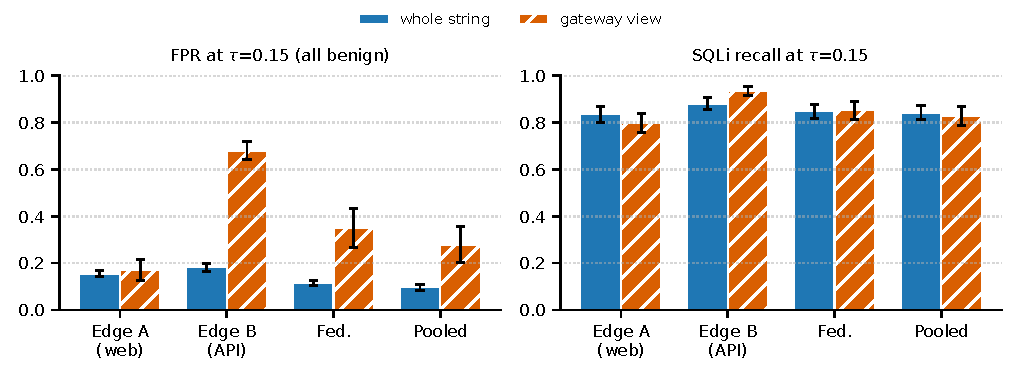
\includegraphics[width=\columnwidth]{figures/fig_deployed.pdf}
\caption{False-positive rate and SQLi recall at $\tau=0.15$ for the retrained recipe, cluster split, 20 seeds, 95\% intervals (\texttt{eval\_deployed\_results.json}). The whole-string and gateway views score the same payloads; only the gateway view takes the maximum over request contexts.}
\label{fig:eval-deployed}
\end{figure}

\paragraph{Ranking in the whole view.}
With grouped splits the three trained models are close and below their exact-unique values: federated ROC-AUC is 0.959 on the cluster split and 0.967 on the random split. Table~\ref{tab:eval-paired} gives the paired differences. Against the silo that validation selects (Edge~B in 15 of 20 cluster seeds) the federated AUC gain is $+0.0021$ with an interval that contains zero; against the silo that turns out best on test it is $-0.0019$ ($-0.0032$ to $-0.0006$); against the pooled model it is $+0.0003$ (interval containing zero) in the cluster mode. Federation matches centralised training in AUC and in recall at the validation-selected 1\% FPR (SQLi difference $0.000$), which is the benchmark the earlier studies lacked: on this data federation gives up nothing to pooling, and gains nothing over it either. Against the selected silo it improves SQLi and XSS recall at 1\% FPR by 0.013 to 0.025 in every split mode, and lowers false positives at $\tau=0.15$ by 0.037 to 0.069 absolute. The one place where the federated model is measurably worse than the alternative is against pooling at the deployed threshold: its FPR is higher by 0.017 (0.003 to 0.032) on the cluster split.

\begin{table*}[t]
\centering
\caption{Federated minus baseline, paired over 20 seeds, whole-string view, with 95\% intervals (\texttt{eval\_deployed\_results.json}). ``Selected silo'' is chosen by validation ROC-AUC; ``best silo'' is the test-optimal one and is optimistic for the silo. Recall at the validation-selected 1\% FPR threshold; FPR at $\tau=0.15$.}
\label{tab:eval-paired}
\begin{tabular}{@{}lccccc@{}}
\toprule
\textbf{Split} & \textbf{AUC vs.\ selected} & \textbf{AUC vs.\ best} & \textbf{AUC vs.\ pooled} & \textbf{SQLi vs.\ selected} & \textbf{FPR vs.\ selected} \\ \midrule
random & $-.0004$ ($-.0014$, $+.0007$) & $-.0004$ ($-.0014$, $+.0006$) & $+.0002$ ($.0000$, $+.0003$) & $+.025$ ($+.017$, $+.033$) & $-.069$ \\
cluster & $+.0021$ ($-.0013$, $+.0055$) & $-.0019$ ($-.0032$, $-.0006$) & $+.0003$ ($-.0001$, $+.0006$) & $+.024$ ($+.015$, $+.033$) & $-.056$ \\
source & $+.0041$ ($+.0011$, $+.0070$) & $-.0004$ ($-.0025$, $+.0017$) & $.0000$ ($-.0003$, $+.0003$) & $+.020$ ($+.007$, $+.033$) & $-.037$ \\ \bottomrule
\end{tabular}
\end{table*}

\paragraph{The deployed threshold.}
The deployed value is not a conservative one. At $\tau=0.15$ the federated recipe flags 11.4\% of benign whole strings (cluster split; interval 10.3--12.5\%), where the validation-selected 1\% budget would flag 1.0\%. In exchange it recovers SQLi recall of 0.848 against 0.766 at the 1\% budget. Because every benign string is a path token, an 11\% rate is not an estimate of production behaviour; the CSIC result below suggests it is a lower bound.

\paragraph{The serving view.}
Scoring by context changes the ranking. Federated AUC falls from 0.959 to 0.921; the FPR at $\tau=0.15$ rises from 0.114 to 0.349 (interval 0.267--0.432), and Edge~B, trained only on API strings, goes from 0.182 to 0.679. The injected-context-only view gives 0.052 for the federated model, so the benign background headers account for most of the excess: the maximum over about four contexts exposes any context that the model scores high on every benign request. In this view the federated model has a higher gateway AUC than the silo selected on validation ($+0.017$, 15 of 20 seeds) only because validation tends to pick Edge~B, the silo that degrades most; Edge~A alone has gateway AUC 0.929 against 0.921 federated. The pooled model is better than the federated one in this view by 0.0009 ($-0.0014$ to $-0.0003$ for federated minus pooled). Which silo a site would have trained, and which view it serves, decide whether federation looks like a gain. A synthetic benign background already produces a 35\% false-positive rate at the deployed threshold; the next question is what a real one produces.

\subsection{Real Data: A Deployment Failure}
\label{sec:eval-real}

\subsubsection*{CSIC 2010 through the gateway scorer}


\texttt{real\_data\_eval.py} scores CSIC~2010 requests with the shipped \texttt{fed\_model.json} through the same context extraction as the gateway. The corpus has 72{,}000 normal requests (the training and test files pooled, 36{,}000 each) and 25{,}065 anomalous ones; the files are fetched from a public mirror, and their SHA-256 digests are recorded in the result file. No CSIC string was used in training. The anomalous class mixes all attack types in the dataset (SQLi, XSS, buffer overflow, CRLF injection, path traversal, information gathering, parameter tampering) and carries no sub-type label, so recall on it is not attack-family recall.

\begin{table}[t]
\centering
\caption{CSIC 2010 through the gateway scorer with the shipped model (\texttt{real\_data\_results.json}); fraction of requests flagged at $\tau=0.15$. ``All contexts'': maximum over path, query, \texttt{User-Agent}, cookie and body, as deployed. ``Payload only'': query and body. Last column: normal requests at threshold~0.5. Counts: 72{,}000 normal, 25{,}065 anomalous.}
\label{tab:eval-csic}
\small
\begin{tabular}{@{}lrrr@{}}
\toprule
\textbf{Scorer} & \textbf{Normal} & \textbf{Anomal.} & \textbf{Normal, 0.5} \\ \midrule
All contexts (gateway) & 1.000 & 1.000 & 1.000 \\
Payload only & 0.191 & 0.523 & 0.167 \\ \bottomrule
\end{tabular}
\end{table}

\begin{figure}[t]
\centering
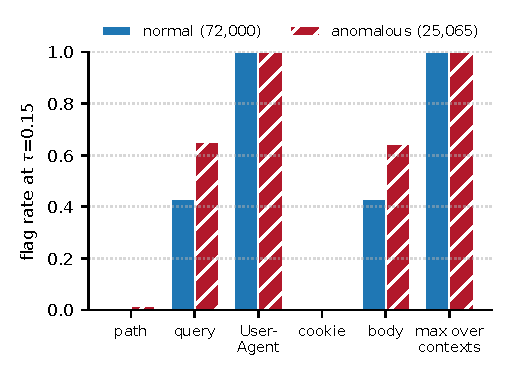
\includegraphics[width=0.85\columnwidth]{figures/fig_csic.pdf}
\caption{Fraction of CSIC~2010 requests whose context scores at least $\tau=0.15$, by context and for the gateway maximum, shipped model (\texttt{real\_data\_results.json}). The \texttt{User-Agent} context is flagged for every request of both classes.}
\label{fig:eval-csic}
\end{figure}

The gateway flags every normal CSIC request at both thresholds: 72{,}000 of 72{,}000 at 0.5 and at 0.15, with a Wilson 95\% lower bound of 0.99995. It also flags every anomalous request, so the full-context decision carries no information about the label (ROC-AUC 0.586, bootstrap interval 0.583--0.589; at the threshold that gives 1\% FPR on normal traffic, recall is 7.9\%). The cause is a single string. All requests in the dataset carry the same \texttt{User-Agent}, \texttt{Mozilla/5.0 (compatible; Konqueror/3.5; Linux)\allowbreak{} KHTML/3.5.8 (like Gecko)}, which the model scores at 0.9992. We did not isolate why the model scores it so high; the string is long and punctuation-dense, features the classifier plausibly associates with attacks. Whatever the reason, the maximum rule turns one repeated header into a deterministic block on every request. The other contexts are not the problem: the 28 distinct normal paths are never flagged (0 of 72{,}000), and none of 36{,}000 distinct normal cookie values reaches 0.15.

Removing the header does not repair the scorer. Over the attacker-controlled contexts only (query and body), 19.1\% of normal requests are flagged at 0.15 and 16.7\% at 0.5, against 52.3\% and 44.9\% of anomalous requests (ROC-AUC 0.695, interval 0.690--0.698). Queries and bodies of normal requests are flagged at 43\% at $\tau=0.15$ (6{,}880 of 16{,}000 queries and 6{,}879 of 16{,}000 bodies); for anomalous requests the figures are 65\% and 64\%. At a deployed threshold chosen on the word lists, roughly one normal request in five would be blocked even if the header were exempted, and the deployed maximum blocks all of them.

This failure was not invisible in Section~\ref{sec:eval-deployed}: the gateway view of the retrained recipe already inflated false positives roughly sevenfold over the injected-context view, through benign background headers. The synthetic background was too mild a test; a real client's constant, long header is a worse one. It also does not show that the classifier is useless on HTTP payloads, only that the scoring and threshold protocol was never validated on any benign string outside the word lists.

\subsubsection*{Synthetic benign probes}

\texttt{real\_data\_eval.py} also scores 3{,}500 deterministically generated, hand-designed benign strings, one context each, in seven categories: names with apostrophes, search text, JSON bodies, base64 and JWT tokens, URLs with query strings, identifiers, emails and addresses, and IoT telemetry paths. These are synthetic and test the generator's assumptions as much as the model. The shipped model flags 37.0\% of them at 0.5 and 51.3\% at $\tau=0.15$ (1{,}797 of 3{,}500). The rate is concentrated: JSON bodies 98\%, query-string URLs 97\% and IoT telemetry paths 98\% at 0.15, against 4.8\% for base64 and JWT, 16\% for search text and 27\% for names with apostrophes. A further category of benign strings that contain SQL keywords, markup and operators in prose (500 strings) is flagged without exception at both thresholds and is excluded from these aggregates. Structured benign data, which is what an API or IoT gateway carries, is the class on which the model fails.

\subsubsection*{Leave-one-corpus-out}

If structured benign traffic is the weak side, how does the attack side generalise beyond the lists the model saw? The leave-one-corpus-out study retrains a centralised model (shipped features, augmentation and hyper-parameters, 600 epochs, three seeds) with one source file, or one whole family, removed from training and scores the removed strings with one random wrapper each. These folds measure generalisation to a new source, not federation. Held-out payloads are exact-deduplicated against training; near-duplicates are not removed.

On the in-distribution reference, attack recall is 0.829 at threshold 0.5 (interval 0.815--0.842) and 0.941 at 0.15, with benign FPR of 0.001 and 0.101. Holding out an entire family cuts recall sharply. When all 17 SQLi lists (681 strings) are removed, recall on them is 0.397 at 0.5 and 0.611 at 0.15 (0.579--0.642); for all 7 XSS lists (523 strings) it is 0.618 and 0.839. Single files vary widely at 0.15: the large \texttt{Generic-SQLi.txt} (260 strings) is recalled at 0.635, \texttt{quick-SQLi.txt} at 0.866 and \texttt{XSS-BruteLogic.txt} at 0.888, while 15 of the 24 attack files are recalled at 0.98 or above. Held-out benign sources show the cost of the lower threshold: the unseen web word list is flagged at 0.9\% at 0.5 and 25.2\% at 0.15 (interval 24.1--26.2\%), the unseen API lists at 0.4\% and 19.4\%. The deployed threshold buys recall on new attack sources at a price in false positives that the in-distribution test did not reveal. The remaining question is whether the learned model can be corrupted, and how much of the damage the aggregation can contain.

\subsection{Byzantine Resilience}
\label{sec:eval-byzantine}

\subsubsection*{Bare aggregators, one seed}


\texttt{poisoning\_\allowbreak experiment.py} is the simplest test. It uses $K=7$ nodes on the domain-split $n$-gram configuration ($\dim=259$, seed~42, 12 rounds, 20 local epochs). From round~4, $f=2$ nodes upload $-12\,w_k$ in place of their weights. Each round the same uploads are aggregated by mean, coordinate-wise median and trimmed mean ($\beta=2$) and scored on held-out payloads (\texttt{poisoning\_results.json}). This script applies no norm gate or authentication: it is an ablation of the bare aggregation rules, not of the deployed pipeline, and it uses one seed.

\begin{figure}[t]
\centering
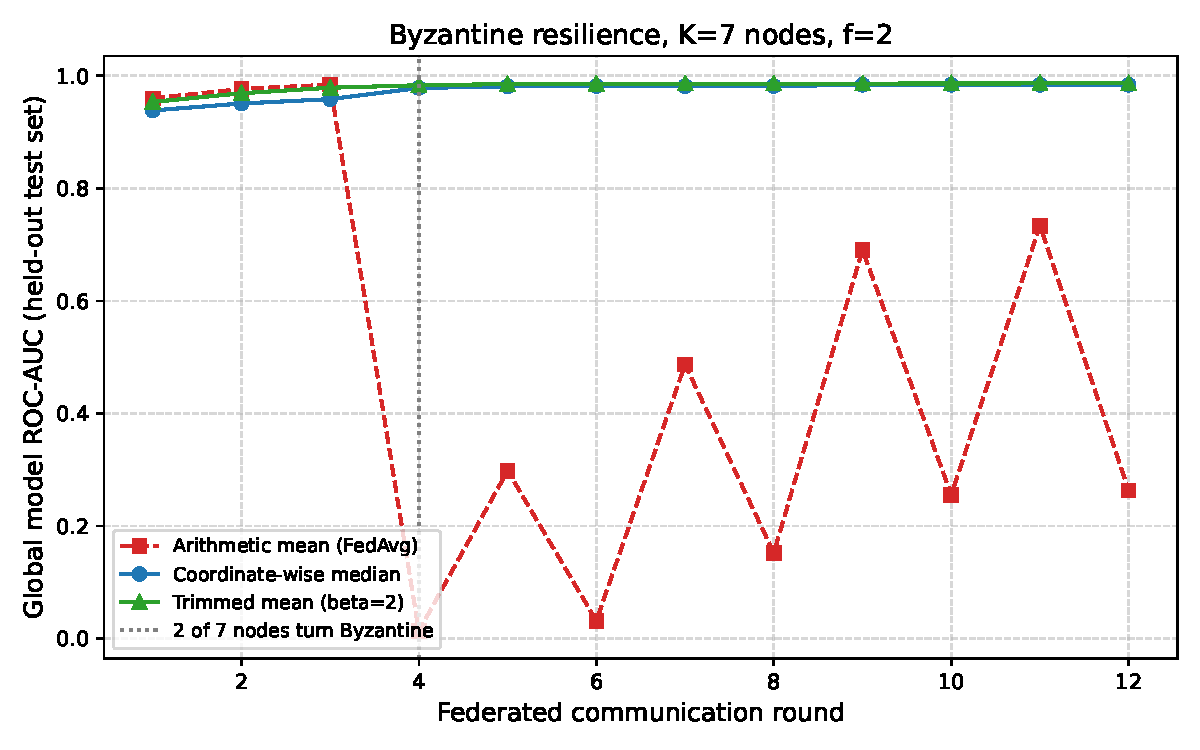
\includegraphics[width=0.95\columnwidth]{figures/poisoning_defense.pdf}
\caption{Bare-aggregator ablation, one seed (\texttt{poisoning\_experiment.py}, no norm gate): from round~4, two of seven nodes upload sign-flipped, $12\times$ amplified weights.}
\label{fig:eval-poison}
\end{figure}

\begin{table}[t]
\centering
\caption{Global-model ROC-AUC in the bare-aggregator ablation (\texttt{poisoning\_results.json}, one seed, no gate); the attack starts in round~4.}
\label{tab:eval-poison}
\begin{tabular}{@{}lccc@{}}
\toprule
\textbf{Aggregator} & \textbf{Round 3} & \textbf{Round 4} & \textbf{Round 12} \\ \midrule
Mean (FedAvg) & 0.984 & 0.014 & 0.263 \\
Coordinate median & 0.958 & 0.978 & 0.984 \\
Trimmed mean ($\beta{=}2$) & 0.979 & 0.983 & 0.986 \\ \bottomrule
\end{tabular}
\end{table}

Averaging falls from 0.984 to 0.014 in the first poisoned round, so the global model is inverted, and ends at 0.263. Median and trimmed mean keep improving, because the two poisoned uploads fall in the trimmed tails of every coordinate. This is the simplest attack in the study, and the deployed norm gate would reject it before aggregation (the next subsection shows exactly that), so Table~\ref{tab:eval-poison} says little about the shipped pipeline.

\subsubsection*{The deployed pipeline under five attacks}

\texttt{poisoning\_v2.py} imports the deployed \texttt{robust\_cloud.norm\_gate} ($\rho=4$) and \texttt{robust\_cloud.aggregate}, so gate and aggregation code are the shipped code. It runs $K\in\{10,20\}$ clients with Dirichlet ($\alpha=1$) non-IID mixes of web, API, SQLi and XSS data and log-normal client sizes, with production augmentation, for 10 rounds and 8 seeds. The malicious fraction goes up to 40\% ($f=4$ of 10; $f=8$ of 20). The attackers are omniscient and collude, and every client is assumed enrolled: authentication is out of scope, so $f$ is bounded by enrolment. The attacks are the $-12\times$ sign flip, ALIE of Baruch et al.\ (2019), a per-coordinate shift of the honest mean by $z$ honest standard deviations against its sign, with $z$ set from $K$ and $f$, the full-knowledge attack of Fang et al.~\cite{fang2020} on median and trimmed mean, label flipping at the clients, and a ``norm-bound'' attack that sends the reversed honest-mean direction scaled to 0.95 of the gate limit so that it passes. Each is run with each of mean, median and trimmed mean (trim~1 per side), with the gate on and off. The metrics are final-round ROC-AUC on held-out payloads, and TPR and FPR at the deployed $\tau=0.15$. The local trainer is a numpy SGD with its own hyper-parameters, not the scikit-learn recipe of the earlier sections, so absolute numbers differ from them.

\begin{table*}[t]
\centering
\caption{Poisoning with the deployed norm gate on (\texttt{poisoning\_v2\_results.json}; mean over eight seeds, final-round global model; FPR at $\tau=0.15$ on held-out payloads, median aggregator). The last row is the clean run ($f=0$) at the same $K$. Gate-off values are in Fig.~\ref{fig:eval-poison-v2}.}
\label{tab:eval-poison-v2}
\begin{tabular}{@{}lccccccccc@{}}
\toprule
 & \multicolumn{3}{c}{\textbf{K=10, f=2 (20\%)}} & \multicolumn{3}{c}{\textbf{K=10, f=4 (40\%)}} & \multicolumn{3}{c}{\textbf{K=20, f=8 (40\%)}} \\
\textbf{Attack} & mean & median & FPR & mean & median & FPR & mean & median & FPR \\ \midrule
Sign-flip & 0.967 & 0.964 & 0.03 & 0.966 & 0.962 & 0.05 & 0.969 & 0.968 & 0.02 \\
ALIE & 0.967 & 0.966 & 0.06 & 0.964 & 0.953 & 0.28 & 0.967 & 0.957 & 0.54 \\
Fang & 0.945 & 0.958 & 0.03 & 0.867 & 0.901 & 0.25 & 0.858 & 0.924 & 0.24 \\
Label-flip & 0.950 & 0.964 & 0.08 & 0.833 & 0.943 & 0.56 & 0.845 & 0.956 & 0.64 \\
Norm-bound & 0.173 & 0.963 & 0.06 & 0.117 & 0.942 & 0.51 & 0.091 & 0.951 & 0.67 \\ \midrule
None ($f{=}0$) & 0.968 & 0.965 & 0.02 & 0.968 & 0.965 & 0.02 & 0.969 & 0.968 & 0.04 \\ \bottomrule
\end{tabular}
\end{table*}

\begin{figure*}[t]
\centering
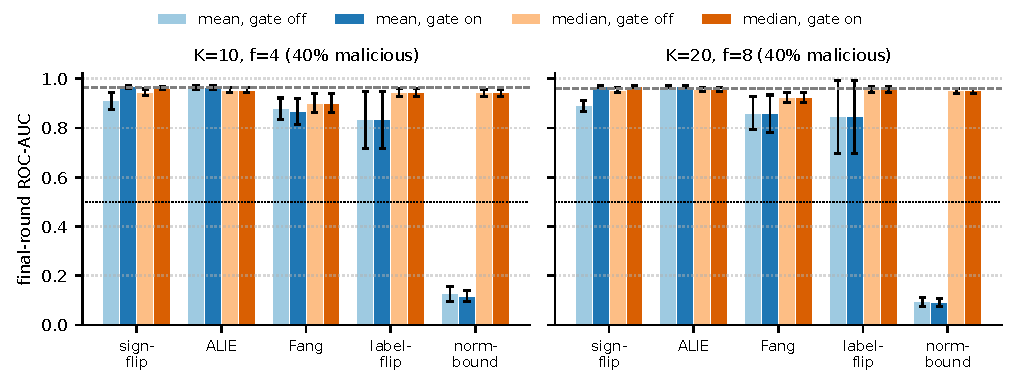
\includegraphics[width=0.85\textwidth]{figures/fig_poison_v2.pdf}
\caption{Final-round ROC-AUC by attack and aggregator, gate off and on, at 40\% malicious clients (left $K{=}10$, $f{=}4$; right $K{=}20$, $f{=}8$), mean $\pm$ 95\% interval over eight seeds (\texttt{poisoning\_v2\_results.json}). Dashed: pooled non-federated reference; dotted: AUC 0.5.}
\label{fig:eval-poison-v2}
\end{figure*}

The gate removes the one attack of the earlier experiment. At $K=10$, $f=2$ with the gate off, the mean aggregator ends at 0.602 $\pm$ 0.258 (its worst round is 0.052) and the trimmed mean (trim~1, which cannot cover two attackers) at 0.463; with the gate on both recover to 0.966 or higher, because the gate rejects every sign-flipped upload (rejection rate 1.00) and no honest one. The median is unaffected by this attack at 20\% malicious (0.963), but at 40\% ($K=10$) it needs the gate: 0.944 with an FPR of 0.49 without it, 0.962 with an FPR of 0.05 with it.

The gate does nothing against the other four attacks, which it rejects at rates of 0 to 0.04. The remaining damage depends on the aggregator and on the fraction, and is more visible in FPR than in AUC. At 20\% malicious the median with the gate stays within 0.958--0.966 AUC for all five attacks at $K=10$, with FPR at 0.15 between 0.03 and 0.08 (clean: 0.02); at $K=20$, $f=4$ the minimum is 0.961 and FPR 0.04--0.15 (clean: 0.04). At 40\% the picture is different. The median's AUC stays at 0.90--0.97, yet under every attack except the sign flip the FPR at $\tau=0.15$ is 0.24--0.67 (0.28 and 0.54 under ALIE at $K=10$ and $K=20$): a model that ranks well but, at the deployed threshold, blocks half the benign traffic. The mean collapses to AUC 0.09--0.17 under the norm-bound attack, which the gate cannot see by construction; the trimmed mean with trim~1 fails the same way at $f=4$ ($K=10$: 0.099) and at $K=20$, $f=4$ (0.886, FPR 1.00), since one trimmed value per side does not cover multiple attackers. No aggregator reaches the clean level under the Fang attack at 40\%, which is the attack designed against it: median 0.901 at $K=10$ and 0.924 at $K=20$.

Two limits qualify these results. First, the evidence concerns a simulation at $K\ge10$; the physical testbed has two gateways and thus $f=0$, where the median of two uploads is their mean (Section~\ref{sec:security}). Second, the AUC-FPR gap just described means that robust aggregation as configured preserves ranking at modest $f$ but not the deployed operating point at large $f$; re-calibrating $\tau$ after each aggregation round is untested.

\subsection{Edge Cost on ARM}
\label{sec:eval-hardware}

\emph{Provenance.} The measurements of this subsection come from the Raspberry~Pi~4 testbed (aarch64 Cortex-A72, 4\,GB; pure-Python gateway on port~8080 with a 15\,s synchronisation interval; load generator \texttt{stress\_test.py}) and are recorded only in the earlier draft \texttt{federated\_paper\_v5.tex}, not in a result file. They predate the final augmentation and the threshold change, which do not alter inference arithmetic. They must be re-measured and archived before the numbers are relied on.

For the 259-coefficient model, inference averages 0.229\,ms per scored string, a single-core ceiling of about 4{,}370\,strings/s, at a resident set of 10.4\,MB dominated by the interpreter. The gateway scores about four contexts per request (Section~\ref{sec:eval-deployed}), so the cost per request is of the order of four times that figure; this is arithmetic on two measurements, not a measurement. Under 1{,}000 requests at concurrency~10, repeated ten times, the threaded gateway sustained $452.5\pm24.3$\,req/s with median latency $20.5\pm0.7$\,ms and 95th percentile $32.2\pm2.5$\,ms and no failed request in 10{,}000. The HTTP stack, not the classifier, was the bottleneck: a single-threaded server serialised keep-alive connections and capped throughput at 42--56\,req/s until \texttt{ThreadingHTTPServer} replaced it. All requests were benign GETs answered with 200; throughput under mixed attack load and for 8\,KB bodies is unmeasured. ML-KEM-512 on the same board cost 0.122\,ms (key generation), 0.162\,ms (encapsulation) and 0.205\,ms (decapsulation) over 1{,}000 warmed-up trials. This is a component benchmark: the live \texttt{/update} and \texttt{/weights} endpoints do not use the derived key.

\subsection{Bandwidth and Data Sovereignty}
\label{sec:eval-bandwidth}

\begin{figure}[t]
\centering
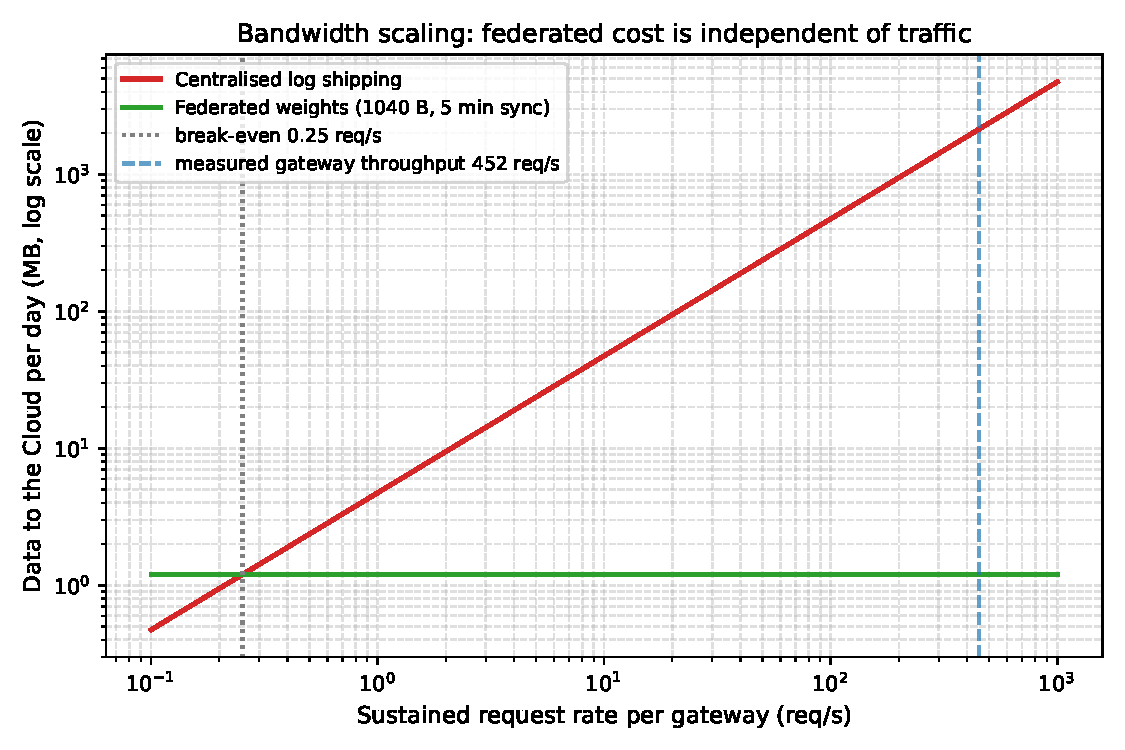
\includegraphics[width=0.95\columnwidth]{figures/fl_bandwidth.pdf}
\caption{Daily traffic to the cloud versus sustained request rate for two gateways (\texttt{bandwidth\_analysis.py}, analytic, 1{,}040\,B per update). The federated cost is flat because each synchronisation carries a fixed-size update.}
\label{fig:eval-bandwidth}
\end{figure}

Bandwidth comparisons commonly set a whole dataset against one update from one node. Here federation is charged for every round, node and direction. The 20-round training run transfers $20\times2\times2\times1{,}040=83{,}200$\,B against 332{,}983\,B of raw request payloads (mean 27.4\,B), a 75.0\% reduction (\texttt{bandwidth\_results.json}). In operation the costs scale differently: log shipping grows with traffic, federation with the synchronisation interval (Table~\ref{tab:eval-bandwidth}).

\begin{table}[t]
\centering
\caption{Daily cloud-bound traffic for two gateways, analytic, 1{,}040\,B per update (\texttt{bandwidth\_results.json}). The 99.94\% figure applies to the 300\,s interval; the deployed interval is 15\,s.}
\label{tab:eval-bandwidth}
\resizebox{\columnwidth}{!}{%
\begin{tabular}{@{}rrrrr@{}}
\toprule
\textbf{Rate} & \textbf{Sync} & \textbf{Centralised} & \textbf{Federated} & \textbf{Reduction} \\ \midrule
10\,req/s & 300\,s & 47.3\,MB & 1.2\,MB & 97.47\% \\
100\,req/s & 300\,s & 473.1\,MB & 1.2\,MB & 99.75\% \\
452\,req/s & 300\,s & 2{,}138.4\,MB & 1.2\,MB & 99.94\% \\
452\,req/s & 15\,s & 2{,}138.4\,MB & 24.0\,MB & 98.88\% \\ \bottomrule
\end{tabular}}
\end{table}

At the 15\,s interval of the testbed the reduction at 452\,req/s is 98.88\%. The break-even is about 0.25\,req/s per node at 300\,s, below which log shipping is cheaper. Three assumptions limit the comparison. The baseline ships every request's payload only (27.4\,B on average), omitting headers and metadata, but also omitting the sampled or flagged-only shipping a practical deployment would use. The update size is 1{,}040\,B (259 float32 values and a bias), whereas the implementation sends JSON text: the coefficient list in \texttt{fed\_model.json} serialises to 5{,}395\,B. With that size, which is arithmetic on the committed values and not a wire measurement, the 20-round training transfer would be 431{,}600\,B and exceed the raw payloads it replaces by 30\%, and the 15\,s reduction at 452\,req/s would be 94.2\%. And none of the figures covers retransmission, TLS or a post-quantum handshake, which are not in the live path. Federation keeps request content inside the site boundary, which Industrial Data Space governance requires; the bandwidth saving is secondary and depends on the update encoding.

\subsection{Unresolved Limits of the Evidence}
\label{sec:eval-limits}

\paragraph{Benign data.}
Every benign string outside CSIC is a path token or a generated string; no captured traffic from a working site is used. The CSIC result shows that the scorer, not just its threshold, fails on an external benign set, so the false-positive figures of Tables~\ref{tab:eval-detection} and~\ref{tab:eval-deployed} should be read as lower bounds.

\paragraph{Operating point.}
The deployed threshold was set on the shipped model and tested here only on retrained models. The shipped model's own held-out behaviour at $\tau=0.15$ has no estimate that is free of training overlap; the CSIC and synthetic-probe results are the only evidence about it, and both are adverse.

\paragraph{Federation gain.}
The advantage of federation over the best silo is below one standard deviation in the exact-unique studies and negative against the test-oracle silo in the cluster split; against pooled training it is nil. What remains is protection against the silo trained on the wrong benign domain and a lower false-positive rate at the deployed threshold than either silo, but a higher one than pooling.

\paragraph{Scale and attacks.}
The detection experiments use $K=2$ nodes with attack data drawn from one shared pool in the domain axis. The poisoning study reaches $K=20$ in simulation with an omniscient, fixed-strategy adversary; there are no adaptive input-space evasions of the linear model, no backdoors, and a physical $f=0$. Attack classes are limited to SQLi and XSS strings from fuzzing lists with 681 and 523 unique entries, so per-seed recall has a standard deviation of 0.06 at 0.1\% FPR.

The security consequences of the update path itself, which these experiments assume and do not exercise, are the subject of Section~\ref{sec:security}.
\emergencystretch=0pt

\section{Security Analysis}
\label{sec:security}

The evaluation leaves a question the accuracy numbers cannot answer: if the gateways and the aggregator are exposed to adversaries, how much of the measured benefit survives, and which parts of the system are actually defended? The answer depends on whom the system trusts, so the adversaries and assumptions come first. They are stated here once; Section~\ref{sec:system} describes the mechanisms without repeating them.

\subsection{Threat Model}
\label{sec:sec-threat}
The deployment is two or more edge gateways, each with a Cortex-A72-class CPU, no GPU and a standard-library Python runtime, and one cloud aggregator. Request payloads are private to the site and are never sent to the aggregator. Four adversaries are considered.

\begin{enumerate}
  \item \textbf{A1, application-layer attacker.} Sends injection and cross-site-scripting payloads through a gateway toward upstream services. The gateway classifier is the control under test.
  \item \textbf{A2, network attacker.} Observes, replays, reorders or forges messages between gateway and aggregator, and may record traffic indefinitely. A2 holds no enrolled secret.
  \item \textbf{A3, Sybil attacker.} Reaches the aggregator and tries to register or impersonate identities in order to outnumber honest peers.
  \item \textbf{A4, compromised gateway.} Holds a valid enrolled secret and uploads arbitrary parameters; it is a Byzantine client, and up to $f$ such nodes are assumed.
\end{enumerate}

The aggregator is trusted to run the aggregation rule and to keep enrolled secrets, but receives no raw payloads. Out of scope are a compromised aggregator and adaptive input-space evasion of the classifier (Section~\ref{sec:sec-limits}). Poisoning optimised against the aggregation rule~\cite{fang2020} is examined only in simulation (Section~\ref{sec:eval-byzantine}). The gateway does not authenticate the clients whose requests it inspects. A1 is handled by classification alone, which is why the paper treats the gateway as a payload-inspection enforcement point inside a zero-trust deployment and not as a zero-trust architecture.

The controls are ordered by what each makes possible for the next. Authentication bounds the number of identities and thereby makes $f$ finite. Admission checks drop malformed or grossly scaled updates before aggregation. Robust aggregation then contains the $f$ Byzantine peers that remain. Without authentication the last layer is void, because an attacker who mints identities controls the median regardless of its guarantee.

\subsection{Poisoning Defence}
\label{sec:sec-poison}
Coordinate-wise median and $\beta$-trimmed mean~\cite{yin2018} (see also Krum~\cite{blanchard2017}) resist Byzantine updates only while honest clients outnumber Byzantine ones in every coordinate:
\begin{equation}
  K \ge 2f + 1 .
  \label{eq:security:byz-bound}
\end{equation}
On the two-gateway testbed $K=2$ gives $f=0$, since the median of two values is their mean and a single Byzantine node is half the population. The aggregator therefore computes $f=\lfloor (K-1)/2\rfloor$ from the number of distinct enrolled peers that have reported and returns it with the model, so that no gateway is told it is protected when it is not. Updates are keyed by client identity and only the latest per peer is kept, so the median runs across peers. An earlier version used a window of the last ten uploads regardless of sender, which is a median over time; a persistent attacker then simply fills a fixed share of the window.

The $\ell_2$-norm gate rejects with HTTP~409 any update whose norm differs from the reference by more than a factor of $4$ (Section~\ref{sec:sys-agg}). It stops gross rescaling. It does not detect sign-flips of ordinary magnitude, nor an update shaped to stay just inside the ratio.

Section~\ref{sec:eval-byzantine} reports two simulations. The first, a bare-aggregator ablation with seven nodes and a $-12\times$ sign flip, bypasses the norm gate and is not evidence about the deployed pipeline. The second runs the shipped gate and aggregation code against five attacks at $K\in\{10,20\}$ and up to 40\% malicious clients, with eight seeds. Two results matter for the argument above. The gate rejects every sign-flipped update and no honest one, and is blind to the other four attacks. The median keeps the ranking quality of the global model at $K\ge 2f+1$ but not its operating point: at 40\% malicious clients the bound still holds ($K=10$, $f=4$ gives $2f+1=9$; $K=20$, $f=8$ gives $17$), yet the false-positive rate at $\tau=0.15$ reaches 0.24--0.67 under four attacks. The bound therefore guarantees bounded influence on each coordinate, not an unchanged decision threshold.

\subsection{Authentication Properties}
\label{sec:sec-auth}
An update passes, in order: enrolment lookup, constant-time MAC comparison, timestamp within $120$\,s, nonce unseen in $300$\,s, per-identity rate limit, dimension and finiteness check (HTTP~400), norm gate (HTTP~409), and finally aggregation. The first failure rejects the update. Unknown and malformed identities receive the same response, so the endpoint does not reveal which identifiers are enrolled. The replay nonce is consumed during verification, before the rate limiter runs, so an update that draws a 429 cannot be resent verbatim. HMAC gives authenticity and freshness; it does not hide the update from an observer (Section~\ref{sec:sec-limits}).

\subsection{Test Plan for the Control Plane}
\label{sec:sec-attacks}
\texttt{test\_auth\_attacks.py} contains ten cases, each built so that a correct control plane returns one specific status code, and run against a live aggregator. The harness rebuilds every message instead of resending it, so a retry past a 429 cannot trigger the replay guard and mask the case under test, and the one case meant to be accepted replays the current global weights, leaving the deployed model unchanged. The repository holds no archived output from a run. Table~\ref{tab:security:attacks} is therefore a test plan with expected verdicts, not a record of passes.

\begin{table}[t]
  \centering
  \caption{Planned control-plane test cases and the status code a correct aggregator should return (not an archived result).}
  \label{tab:security:attacks}
  \small
  \begin{tabular}{@{}p{3.0cm}@{\hspace{4pt}}c@{\hspace{4pt}}p{1.7cm}@{\hspace{4pt}}p{1.2cm}@{}}
    \toprule
    Case & Expect & Control & Threat \\
    \midrule
    Untagged update (old format); unknown self-tagged identity & 401 & enrolment, MAC & A2, A3 \\
    Forged tag; tampered weights with stale tag & 401 & MAC & A2 \\
    Replay of an accepted update; timestamp one hour old & 401 & nonce, clock & A2 \\
    Second update inside rate window & 429 & rate limit & A4 \\
    $50\times$ scaled weights & 409 & norm gate & A4 \\
    Wrong dimension; NaN weights & 400 & validation & A4 \\
    \bottomrule
  \end{tabular}
\end{table}

Even a clean run would show only that each control returns its designed verdict. It would not establish security, and it says nothing about plausible-norm, adversarially chosen weights from an enrolled node.

\subsection{Hardening Changes}
\label{sec:sec-audit}
A code review against the draft claims produced changes that bear on how earlier numbers are read. The original poisoning figure had been drawn from hard-coded values and was replaced by a measurement. The Byzantine argument had been void at $K=2$ and the update window was keyed by time rather than peer; both are fixed and $f$ is now reported. One model file replaces three inconsistent models. Handlers reject a missing or non-numeric \texttt{Content-Length} with HTTP~400, servers use \texttt{ThreadingHTTPServer} with a $5$\,s connection timeout, counters are updated under locks, and model snapshots are published by write, \texttt{fsync} and \texttt{os.replace}. Lowering the block threshold from $0.5$ to $0.15$ after data augmentation is an operating-point change, not a security fix; its false-positive cost is examined in Section~\ref{sec:eval-deployed}.

\subsection{Limitations}
\label{sec:sec-limits}
\paragraph{Byzantine tolerance at deployed scale.}
Two gateways give $f=0$ by~\eqref{eq:security:byz-bound}, and the poisoning results come from simulation. Authentication and the norm gate still apply at $K=2$, but neither stops a compromised gateway that uploads plausible-norm weights chosen adversarially.

\paragraph{Adaptive attacks.}
The simulation includes one aggregation-aware attack, the full-knowledge attack of Fang \textit{et al.}~\cite{fang2020}, and no adaptive timing, backdoors or collusion beyond a fixed strategy. The classifier is linear over hashed trigrams and simple syntactic features, and padding, entropy shaping or steering trigrams toward lightly weighted buckets can plausibly evade it. No input-space evasion was evaluated, so the poisoning results say nothing about evasion.

\paragraph{Authentication.}
Symmetric keys mean a breach of the aggregator exposes every peer secret, and the scheme offers no non-repudiation. Replay and rate-limit state live in aggregator memory and are lost on restart. Enrolment is manual, which bounds $f$ and also costs operator effort. The timestamp window assumes loosely synchronised clocks.

\paragraph{Confidentiality and privacy.}
Live updates and global models travel as plain-HTTP JSON on a trusted network segment, and the ML-KEM exchange is a standalone benchmark (Section~\ref{sec:sys-pqc}). An observer of the link can read the weights, and a recorded exchange could be read later by a quantum-capable adversary; A2's recording capability is not neutralised. Differential privacy is not implemented, so no $\epsilon$ is reported and gradient inversion was not measured. The parameters an update carries are a function of a site's training data, and what that reveals is unquantified.

\paragraph{Statistical scope.}
The attack tests assert designed status codes and were not run as a study. The bare-aggregator ablation is a single seeded run; the deployed-pipeline sweep has eight seeds and a simulated, omniscient adversary. What the analysis supports is narrow: authenticated, rate-limited, norm-checked updates from enrolled peers, and a median rule that preserves ranking quality under the tested attacks while $K\ge 2f+1$, at a cost in false positives that grows with the malicious fraction.


\section{Conclusion and Future Work}
\label{sec:conclusion}

For a hashed-trigram payload classifier, federation pays off when sites differ in benign traffic: the federated model matches pooled training and the better silo within seed variation, protects the silo whose benign profile is wrong for the test traffic, and does not need to know in advance which silo that is. It does not raise the ceiling set by the best local model or by pooling, and when sites differ in attack mix it lands between the silos. A boosted-tree model on the same features is more accurate than any linear variant, so the linear choice is a cost decision. On the deployment side the results are negative: on CSIC~2010 the gateway rule flags every normal request, so nothing here measures false-positive behaviour on production traffic. The prototype authenticates updates, and its median keeps the ranking of the global model when up to 40\% of simulated clients attack it, but at the deployed threshold it blocks 24--67\% of benign strings at that fraction under four of five attacks. The live channel is unencrypted and the two-gateway testbed has no Byzantine tolerance.

The experiments that would change these conclusions, in order of priority, are: scoring each request context with a threshold calibrated on captured benign traffic from the target site, which addresses the CSIC failure directly; repeating the heterogeneity study with more than two clients and a larger SQL-injection corpus, since 681 unique strings make recall at a 0.1\% false-positive budget unstable across seeds; recalibrating $\tau$ after each robust aggregation and testing evasion aimed at the trigram map; and wiring the ML-KEM-derived key into authenticated encryption of the update channel so that its cost can be measured end to end rather than as a component.

\section*{Acknowledgment}
This work was partially supported by the Swedish Knowledge Foundation (KK-stiftelsen) and the Mid Sweden University Industrial IoT research initiative.

\section*{Data and Code Availability}
The dataset manifests, federated simulation, Byzantine poisoning experiment, pure-Python edge inferencer and testbed instructions are available at \url{https://github.com/eldemaster/FedZTA-Edge}.

\bibliographystyle{IEEEtran}
\bibliography{refs}

\end{document}
